\documentclass[conference]{IEEEtran}
\IEEEoverridecommandlockouts
% The preceding line is only needed to identify funding in the first footnote. If that is unneeded, please comment it out.
\usepackage{cite}
\usepackage{amsmath,amssymb,amsfonts}
\usepackage{algorithmic}
\usepackage{graphicx}
\usepackage{textcomp}
\usepackage{xcolor}
\def\BibTeX{{\rm B\kern-.05em{\sc i\kern-.025em b}\kern-.08em
    T\kern-.1667em\lower.7ex\hbox{E}\kern-.125emX}}
    
\graphicspath{ {./images/} }

\begin{document}

\title{Hypothesis: \\ A larger amount of features improves the segmentation performance\\
}

\author{\IEEEauthorblockN{Riccardo Dario Dirnberger}
\IEEEauthorblockA{\textit{Biomedical Engineering} \\
\textit{University of Bern}\\
Bern, Switzerland \\
riccardo.dirnberger@students.unibe.ch}
\and
\IEEEauthorblockN{Niklas Freudiger}
\IEEEauthorblockA{\textit{Biomedical Engineering} \\
\textit{University of Bern}\\
Bern, Switzerland \\
niklas.freudiger@students.unibe.ch}
\and
\IEEEauthorblockN{Severin Albert Willingsdorfer}
\IEEEauthorblockA{\textit{Biomedical Engineering} \\
\textit{University of Bern}\\
Bern, Switzerland \\
severin.willingsdorfer@students.unibe.ch}
}

\maketitle


%\hfill\newpage\hfill\newpage

%%% to generate tables: https://www.tablesgenerator.com/

%%%%%%%%%%%%%%Added a new page just for viewing reasons

%-----------------------------------------------------------------------------------

\begin{abstract}
Medical image analysis, specially Artificial Intelligence (AI) which can segment regions in the body gets more and more important nowadays. Such AI models which segment brain regions, like in this case here, uses features to improve the quality of the segmentation. The hypothesis "A larger amount of features improves the segmentation performance" will be examine in this report and rejected. The performance does not get better with more features in respect of the segmentation quality and time to compute. A random forest calcification is used with the Features Intercity, Gradient-Intensity and Neighbourhood. Further, could be shown that noisy training data makes the segmentation worse.
\end{abstract}

%\begin{IEEEkeywords}
%component, formatting, style, styling, insert
%\end{IEEEkeywords}

%-----------------------------------------------------------------------------------

\section{Introduction} \label{sec:Introduction}
Medical image segmentation is a critical component within the medical image analysis pipeline and the foundation for accurate diagnosis and treatment planning. Manual segmentation is a time-consuming and expensive task; therefore, if possible, automatic image segmentation is employed. Although automated segmentation reduces the time and effort involved, the process itself can still be improved. Image segmentation uses a set of features. Even though more features can enhance segmentation accuracy, they also increase the required time. Hence, it is crucial to progressively incorporate only the feature with the most significant impact until, by their combination, the required segmentation accuracy for a specified problem is achieved. Thus, minimizing the required time for automatic image segmentation. This project compares features for brain region segmentation in relation to their importance for segmentation performance. Thereby providing a guide to effective feature selection, aiming to minimize the trade-off between time consumption and segmentation accuracy of automated image segmentation.
\textcolor{red}{references}

%-----------------------------------------------------------------------------------

\section{Materials \& Methods} \label{sec:Materials \& Methods}
\subsection{MRI Data} \label{subsec:MRI Data}
 The 3 tesla MRI dataset consists of 30 unrelated healthy subjects from the Human Connectome Project (HCP) dataset. For each subject one T1-weighted and one T2-weighted image is available. Both images are not skull-stripped but defaced for anonymisation as well as a bias field correction is applied. Additionally, the brain mask and the ground truth labels, the latter generated by FreeSurfer 5.3, as well as an affine transformation for image to atlas alignment are available per subject \cite{b2}. The data of 20 of the subjects was used for training and the remaining data of 10 of the subjects for testing.

\subsection{MIA Pipeline} \label{subsec:MIA Pipeline}
The medical image analysis (MIA) pipeline consists of the steps shown in Fig.~\ref{fig:MIA pipeline}. The basic pipeline was given to us by our lecturers and only certain steps were modified \cite{b1}. The steps numbered as 1 and 3 were not modified, only at the beginning certain parameters were fixed. The main pipeline modifications were performed in step 2 and 3. Within a the following a short description of each MIA pipeline step is given:

\begin{itemize}
    \item Registration: The registration is applied to the image given a atlas image and a transformation.
    \item Preprocessing: Within the preprocessing skull-stripping and z-score normalisation is applied to the image.
    \item Feature Extraction: A variety of different image features were introduced which can be combined to different feature combinations. A more in depth description is given in subsection~\ref{subsec:Feature Extraction}.
    \item Classification: A Random Forest Classifier is used. The hyper-parameters were manually optimised to a certain extend (good Dice score with acceptable time consumption) at the project start and thereafter fixed (estimators~=~10, depth~=~30). Additionally, the random seed of numpy was fixed to 42 to attain reproducibility.
    \item Postprocessing: As there is no actual postprocessing implemented in the given MIA pipeline, the implemented framework was removed to increase performance.
    \item Evaluation: For the evaluation a variety of testing datasets were used to calculate different metrics. An in-depth description can be found in subsection \ref{subsec:Evaluation}.
\end{itemize}

\begin{figure}[h!]
  \centering
  \includegraphics[width=0.95\linewidth]{images/MIA Pipeline.png}
  \caption{MIA Pipeline}
  \label{fig:MIA pipeline}
\end{figure}
\newpage
\subsection{Feature Extraction} \label{subsec:Feature Extraction}
For the feature extraction five features were used as shown in  Fig.~\ref{fig:Features and Feature Combinations}. The Atlas-Coordinate-Feature~(C) is the base feature and must always be  activated. All other features can respectively be used for T1-weighted (T1w) and T2-weighted (T2w) images individually or combined. The three main features are Intensity~(I), Gradient-Intensity~(G) and Neighbourhood~(NH). The first two are once the pixel values and once the gradient thereof. The Neighbourhood-Feature is a vector consisting of 15 first order texture features~(FOTF) including mean, variance, min and max. The FTOF is calculated over the whole image for a kernel size of 3x3. The last feature is named Noise-Feature~(GA~\&~SP). It is similar to the Intensity-Feature in the sense of it representing the pixel values but with the difference of noise added to the image. The feature is implemented separately for Gaussian-Noise~(GA) and Salt \& Pepper-Noise~(SP) but was always used in combination. The following parameters were used: GA (standard deviation = 500), SP (probability = 0.02).

\begin{figure}[h!]
  \centering
  \includegraphics[width=0.95\linewidth]{images/Feature Combinations.png}
  \caption{Features and Feature Combinations}
  \label{fig:Features and Feature Combinations}
\end{figure}

Out of these features a variety of combinations, in total 13 as shown in Fig.~\ref{fig:Features and Feature Combinations}, were tested for their segmentation performance. Atlas-Coordinate-Feature is used as the baseline. The main features, Intensity, Gradient-Intensity and, Neighbourhood, are once used individually and once combined, for only T1 and only T2 respectively. An additional combination is the fusion of the main features for T1 and T2. The last three combinations are the main features individually with the addition of the Noise-Feature.

\subsection{Evaluation} \label{subsec:Evaluation}
The training of all feature combinations was performed on UBELIX, a high performance computer system of the University of Bern. Each task was submitted with the following parameters: 20~CPUs, multi-core-processing, and 16~GByte of memory.

To evaluate the segmentation quality of the different combinations, the Dice score, Hausdorff-Distance (95th percentile) and weighted Dice score was calculated.
The Dice score is a similarity measurement between two datasets, in our case the segmentation result and ground truth segmentation. The Hausdorff-Distance is the largest distance between the border of the segmentation result and the border of the ground truth segmentation. These two metrics are common tools to evaluate segmentation quality.
The Dice score introduces a bias if the segmented labels have a large difference in volume. More specifically, for labels with small volume the Dice drops significantly if a few voxels are wrongly labeled, whereas for labels with large volume the Dice stays similar. Based on this fact a weighted Dice score (Equation \ref{eq:1}) was introduced, which calculates the Dice score per subject with respect to the volume of each label.

% If two big areas have a displacement of one pixel the Dice score is still high. If a smaller area has the same offset the Dice score is much smaller. That is the reason why the weighted Dice is calculated. This is made as follow:

\begin{equation} \label{eq:1}
weighted\ Dice = \frac{\sum_{n}^{labels} \frac{Dice_n}{volume_n}}{\sum_{n}^{labels} \frac{1}{volume_n}}
\end{equation}

% Equation \ref{eq:1} gives the dice score for each subject back in respect of the area of each label.
Each trained model was evaluated with a testing dataset of ten test subjects. The robustness of the model was evaluated by noise augmentation of the testing dataset. Therefore, the model was not only evaluated with the original testing dataset, but with an additional seven noisy testing datasets. These noisy datasets consist of four datasets with added Gaussian noise with a standard deviation of 300, 1'000, 2'000, and 5'000 and three with added Salt and Pepper noise with a probability of 1\%, 2\%, and 5\%. The highest noise levels for both noise types generate images which can be viewed as extreme cases of noise and thus, would be redone within a clinical setting. The robustness per label was calculated by subtracting the individual noisy dataset from the original dataset and calculating the mean, maximal, and minimal value of the seven attained difference-datasets. Leading to a effective metric for robustness comparison of different feature combination models.


% The evaluation of the trained AI is made with ten testing images. To evaluate how robust each training network is, noise was applied to the test data. Beside the run throw this ten images, seven runs more where made with noise. Salt and Pepper noise was used with a threshold of 1\%, 2\% and 5\% as well as Gaussian noise with sigma equal to 300, 1'000, 2'000 and 5'000. The last noise value of Salt and Pepper and Gaussian are so high that every radiologist would make the image again. So these are extreme cases. Out of this test we got different dice scores. All this dice scores where subtracted from the testing without noise. That results in the robustness. The mean and maximal and minimal value is calculated out of this seven differences. Like this can be shown how robust a model is with different Features.

%-----------------------------------------------------------------------------------

\section{Results} \label{sec:Results}

\begin{figure}[h!]
  \centering
  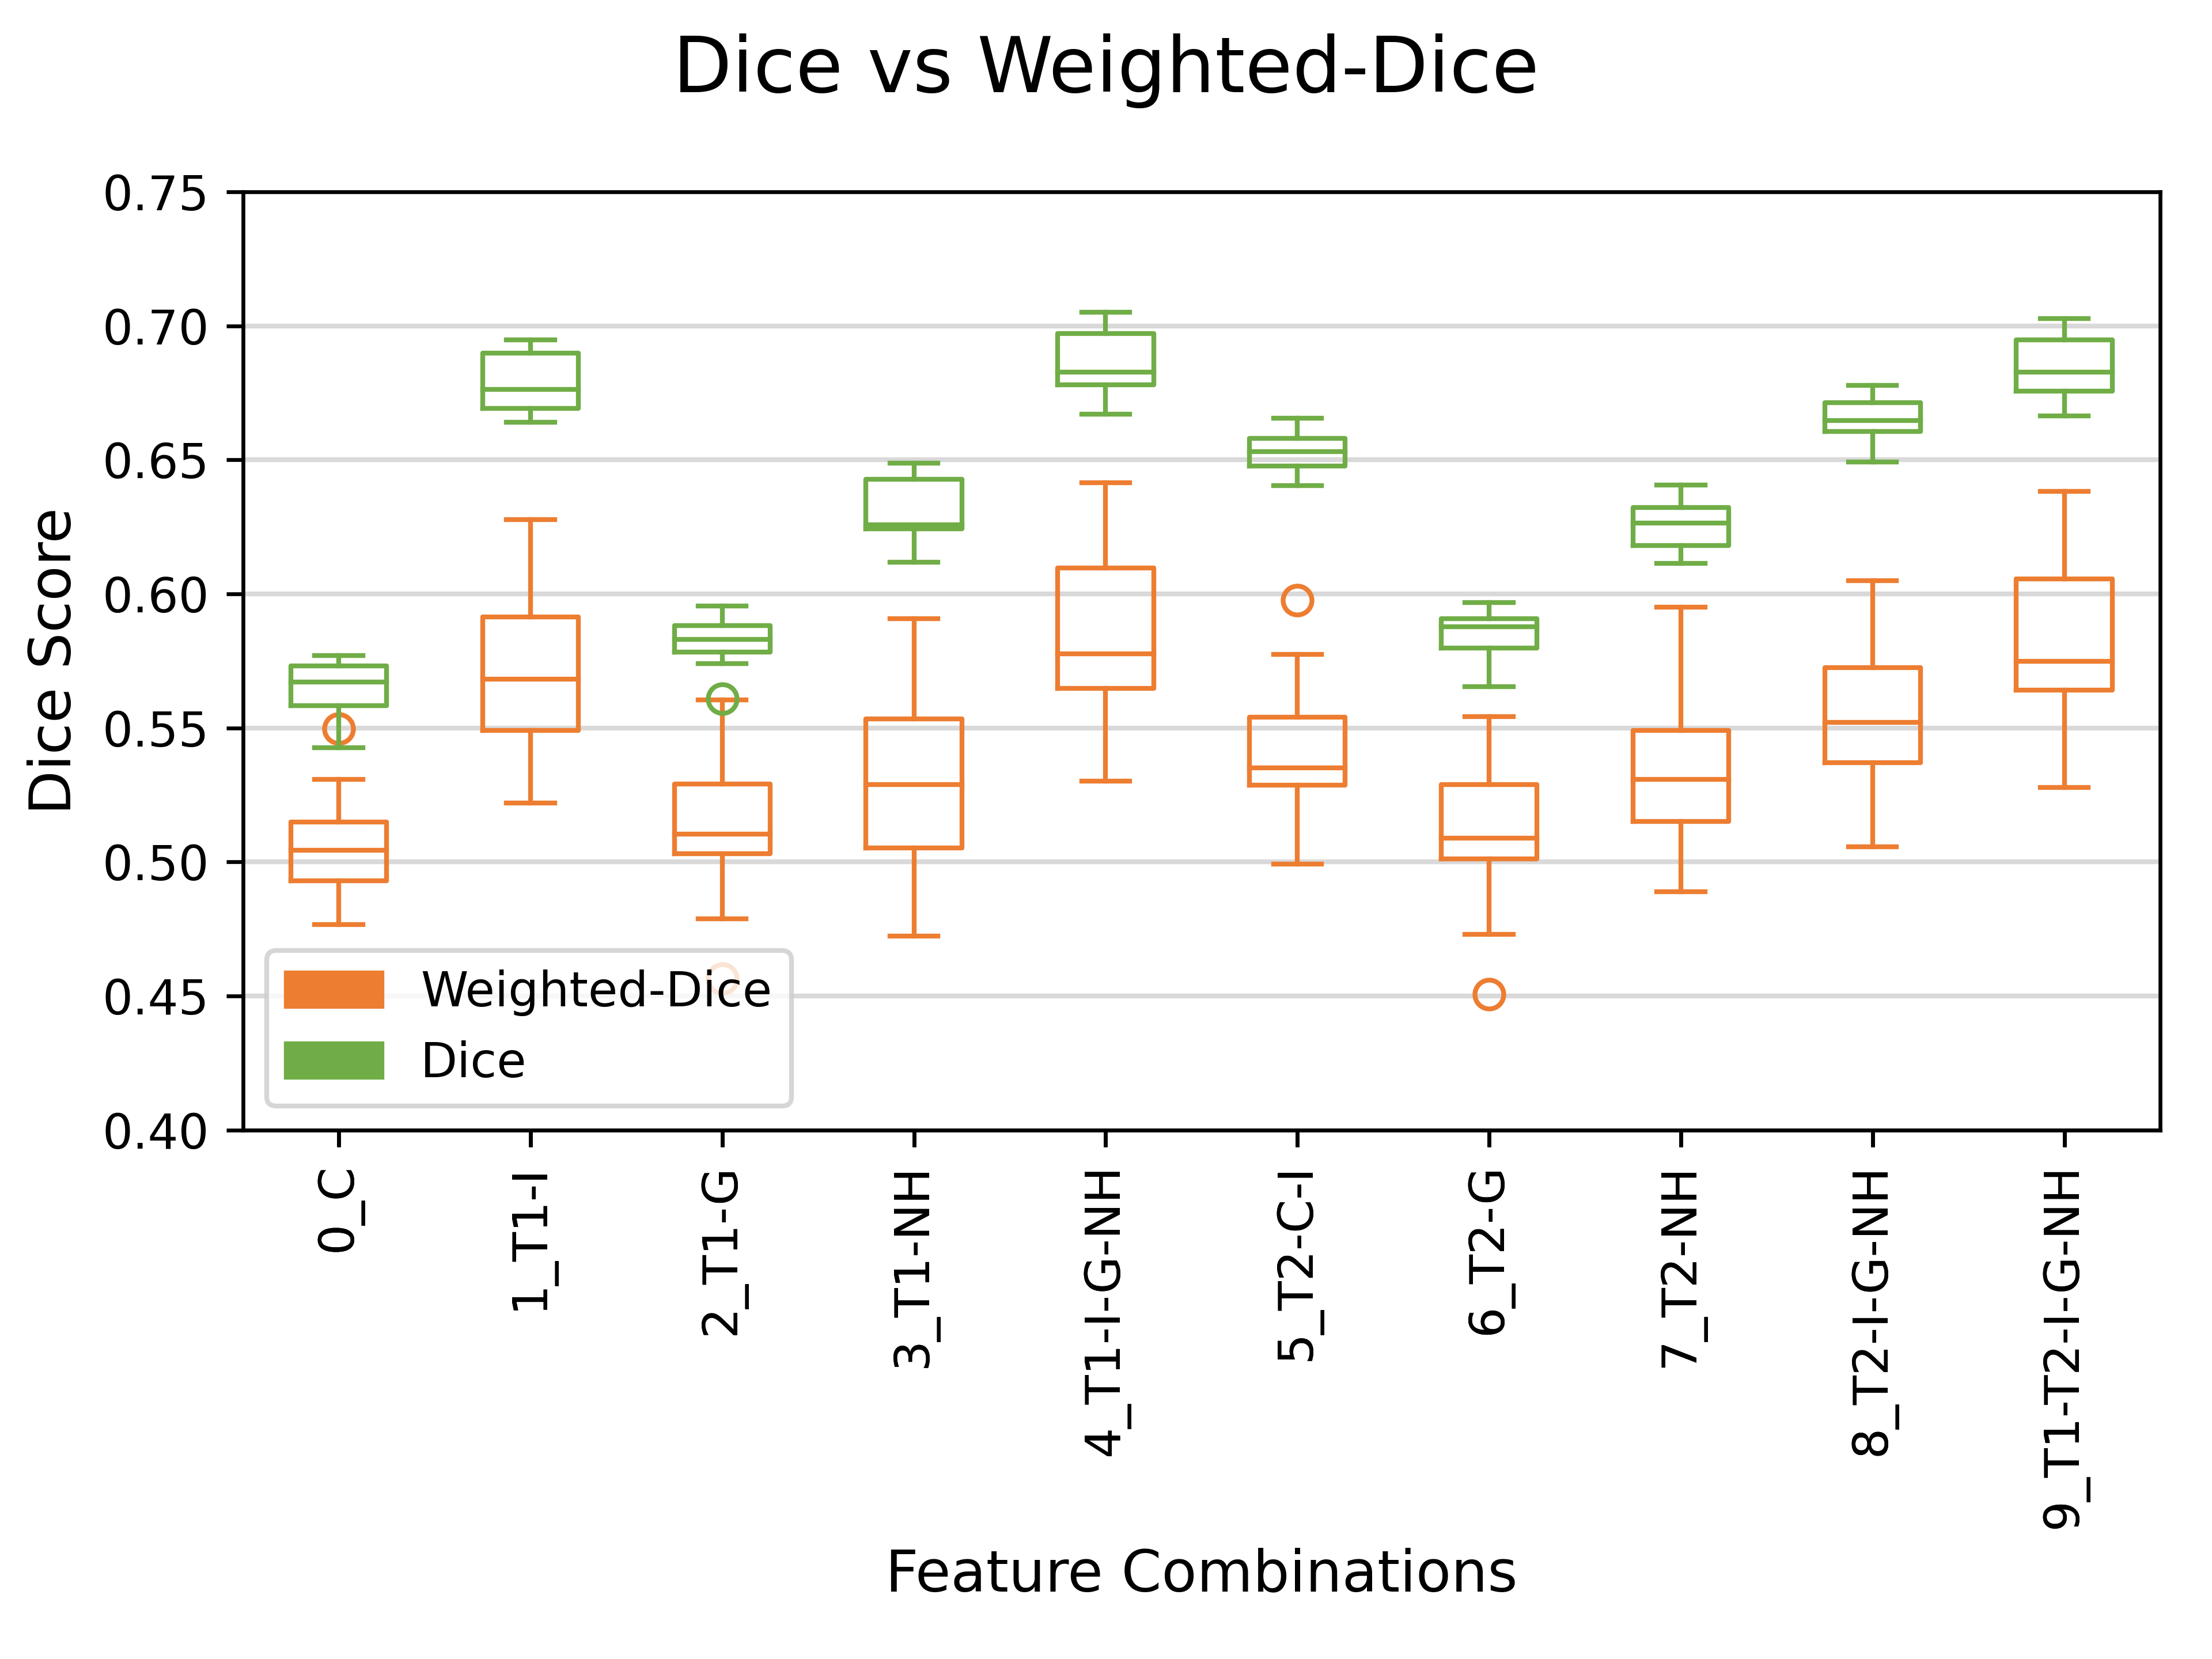
\includegraphics[width=0.95\linewidth, trim={0 4mm 0 10mm}, clip]{diceStuffZoomed}
  \caption{Comparison of Dice and weighted Dice for different feature combinations.}
  \label{fig:diceScore}
\end{figure}

\begin{figure*}[b]
  \centering
  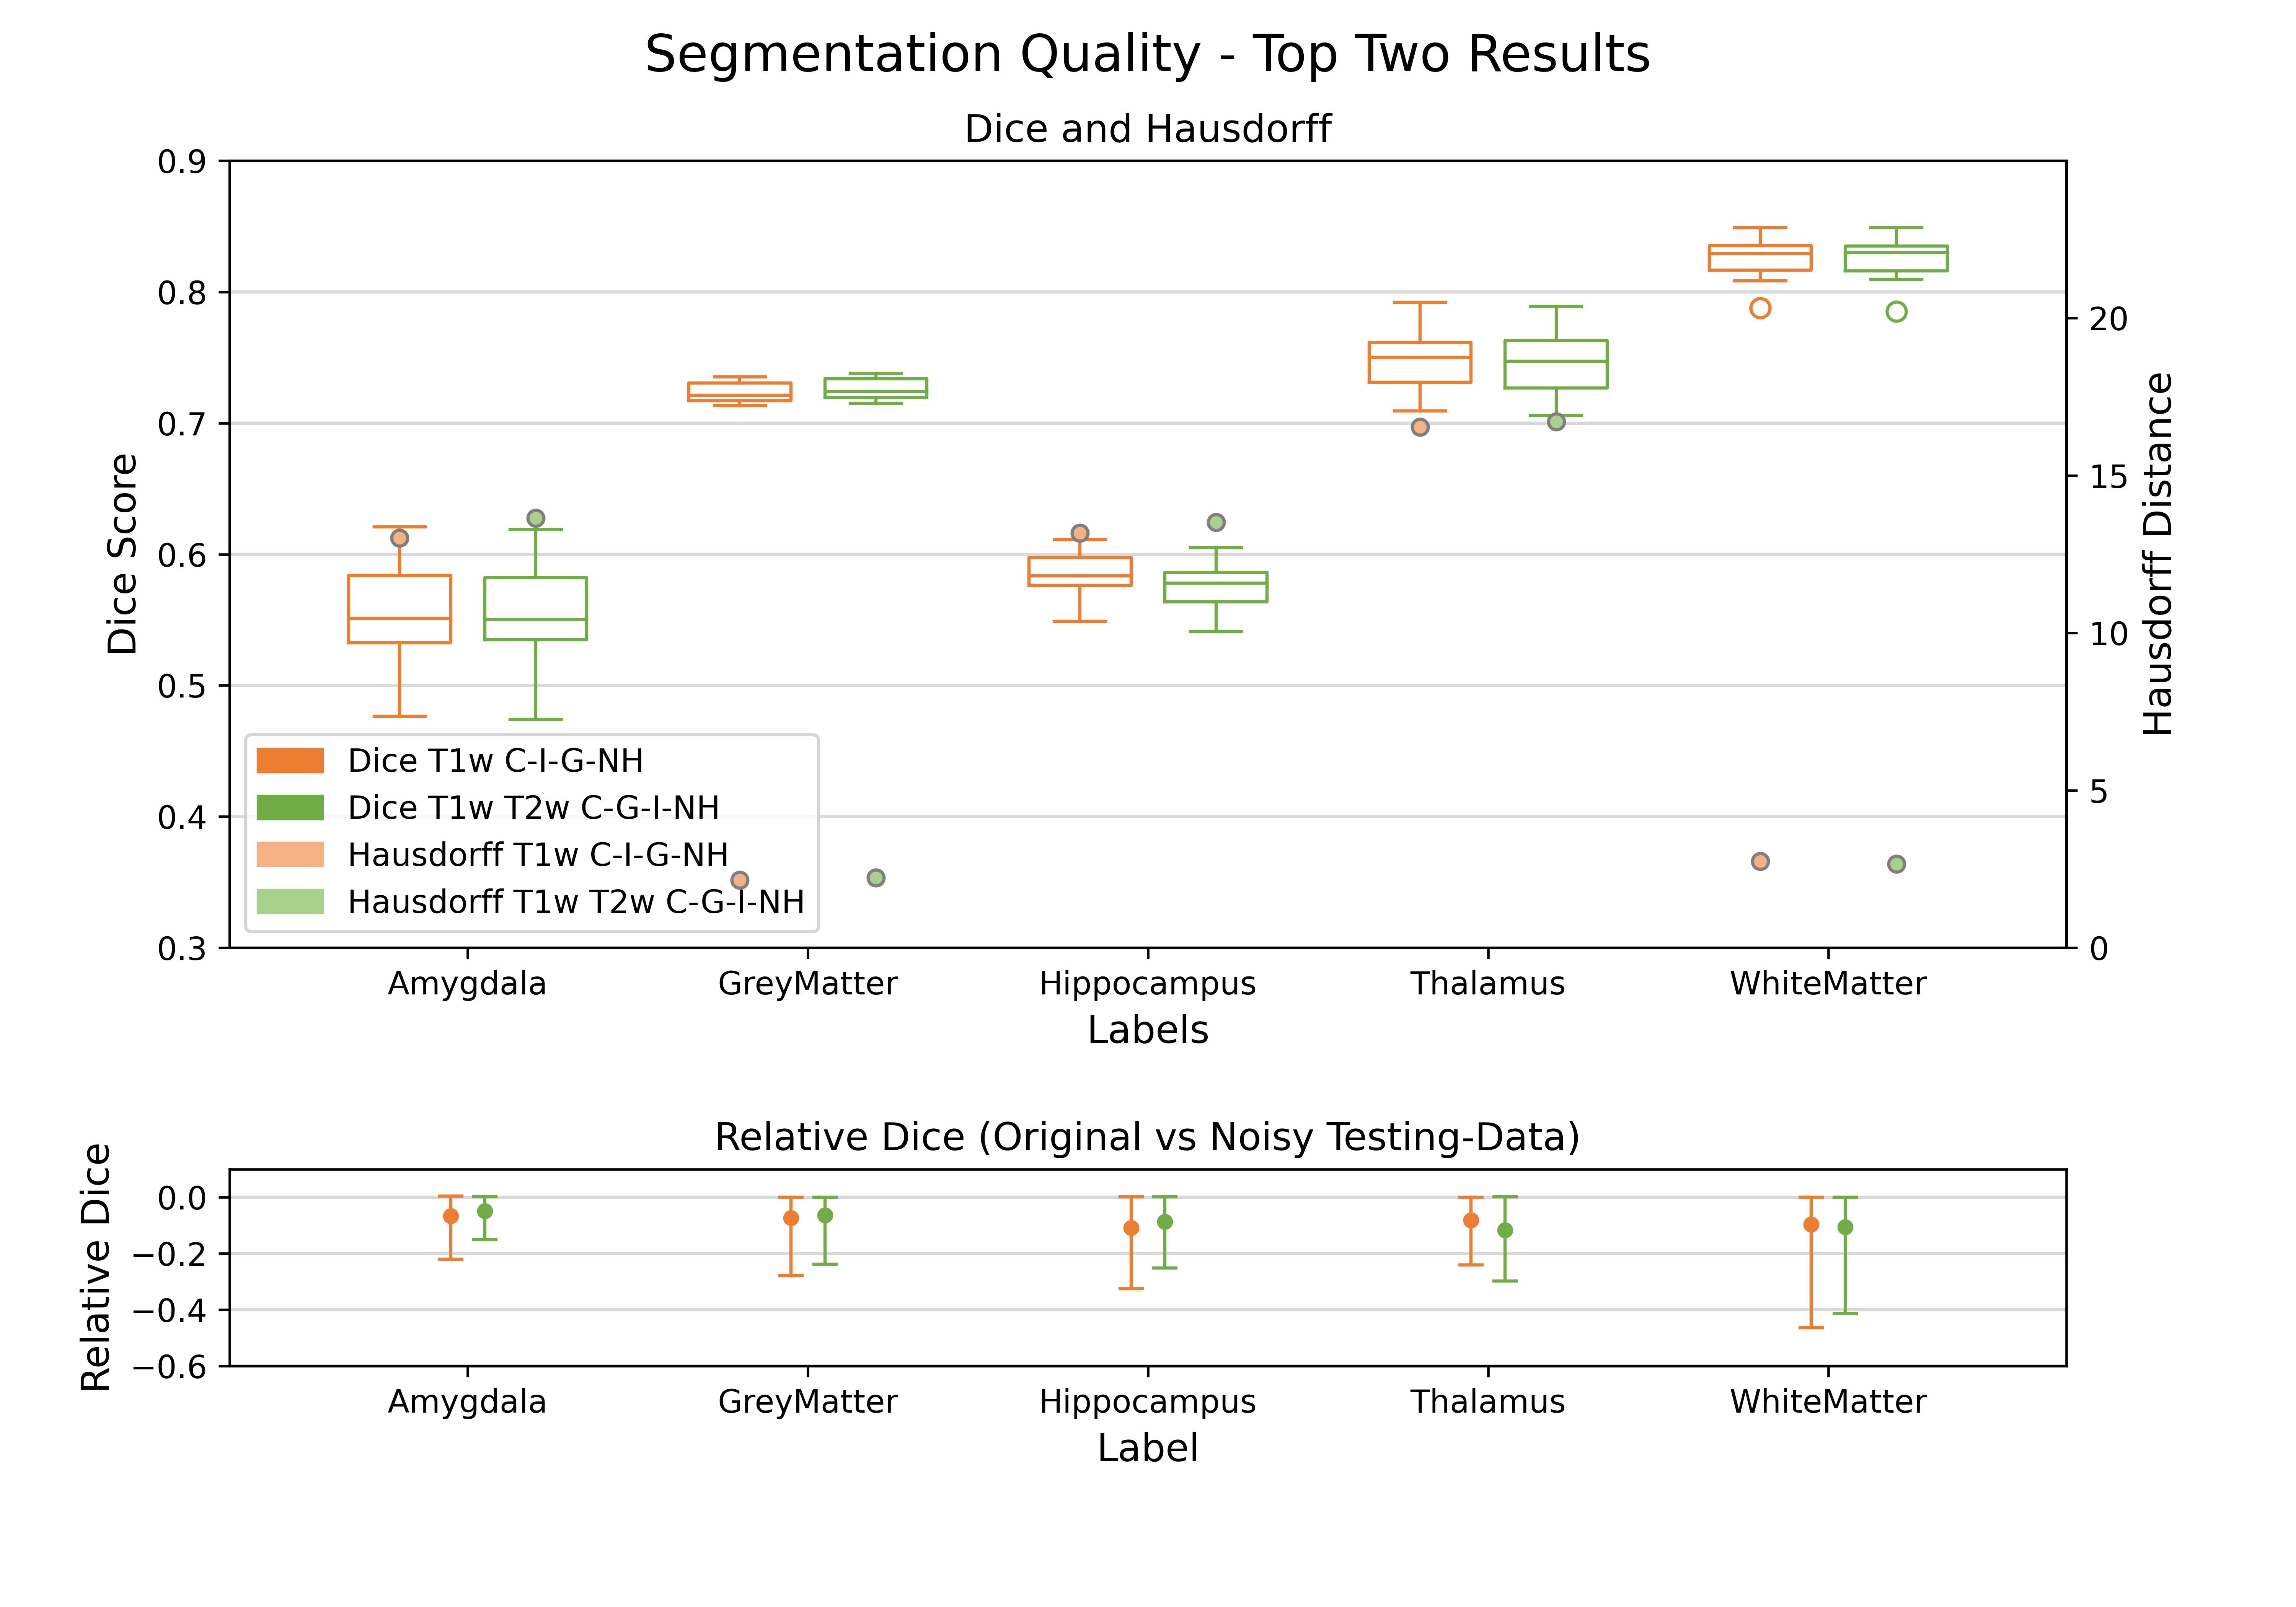
\includegraphics[width=0.95\linewidth, trim={0 8mm 0 10mm}, clip]{04_T1W_C_I_G_NH_and_09_T1W_T2W_C_I_G_NH_zoomed}
  \caption{Direct comparison of the top two feature combinations.}
  \label{fig:bestRun}
\end{figure*}

For comparison of segmentation quality of different feature combinations the results are plotted as boxplots showing Dice and weighted Dice.


To be able to compare the performance of the different features, a plot was made which shows the dice and weighted dice score form all runs we made. Fig.~\ref{fig:diceScore} shows all dice scores form the different labels and subjects where put in one dataset and displayed as a box-plot. The same with the weighted dice score. In general is the distribution of the dice score narrower than from the weighted dice. The offset between the orange and green box-plots is mostly the same so it does not matter if we evaluate on dice or weighted dice. All further evaluation will focus on the dice score.
A lot of data gets lost in a plot like this. To make sure that this comparison is correct, the T1-weighted and T2-weighted results with the same Features where compared \emph{(Appendix)}. These plots shows the same results.
The run number four and run number nine made reach the best dice score in Fig.~\ref{fig:diceScore}. To evaluate which run performed better, a second plot was made Fig.~\ref{fig:bestRun}.



Fig.~\ref{fig:bestRun} shows the performance of the two runs which reached the highest dice score in over all comparison. This plot design is the same as in \emph{(Appendix)}. At the top plot is the dice distribution from each label shown by box-plots. The scale for the dice can be found on the right. On the left side is the scale for the Hausdorff-Distance. This is related to the dots with the gray border. This dots display the mean over all measured distances. The bottom plot shows the robustness. As described in subsection ~\ref{subsec:Evaluation} the robustness is described by the relative dice. The dot shows the mean of the five values and the bar shows the maximal and minimal value.\\

\begin{table}[h!]
\begin{center}
\begin{tabular}{lll}
\textbf{Median}  & \textbf{T1w C-I-G-NH} & \textbf{T1w T2w C-I-G-NH} \\\hline
Amygdala         & 0.5511                & 0.5502                    \\
Grey Matter      & 0.7212                & 0.7241                    \\
Hippocampus      & 0.5834                & 0.5781                    \\
Thalamus         & 0.7500                & 0.7473                    \\
White Matter     & 0.8292                & 0.8299                    \\
                 &                       &                           \\
\textbf{Average} & \textbf{0.6870}       & \textbf{0.6859}           \\
\\
\end{tabular}
\caption{Comparison of the two best Feature combinations according to median dice score form all labels.}
\end{center}
\label{table:Median}
\end{table}


\begin{table}[htbp]
\caption{Table Type Styles}
\begin{center}
\begin{tabular}{|c|c|c|c|}
\hline
\textbf{Table}&\multicolumn{3}{|c|}{\textbf{Table Column Head}} \\
\cline{2-4} 
\textbf{Head} & \textbf{\textit{Table column subhead}}& \textbf{\textit{Subhead}}& \textbf{\textit{Subhead}} \\
\hline
copy& More table copy$^{\mathrm{a}}$& &  \\
\hline
\multicolumn{4}{l}{$^{\mathrm{a}}$Sample of a Table footnote.}
\end{tabular}
\label{tab1}
\end{center}
\end{table}



\begin{table}[h!]
\begin{tabular}{lll}
\textbf{Mean}    & \textbf{T1w C-I-G-NH} & \textbf{T1w T2w C-I-G-NH} \\
Amygdala         & 0.55234               & 0.5518                    \\
Grey Matter      & 0.72339               & 0.7263                    \\
Hippocampus      & 0.58435               & 0.5767                    \\
Thalamus         & 0.74681               & 0.7454                    \\
White Matter     & 0.82521               & 0.8251                    \\
                 &                       &                           \\
\textbf{Average} & \textbf{0.6864}       & \textbf{0.6851}           \\
\\
\end{tabular}
\caption{Comparison of the two best feature combinations according to mean dice score of all labels.}
\label{table:Mean}
\end{table}


To compare the results shown in Fig.~\ref{fig:bestRun}, Table~\ref{table:Median} and Table~\ref{table:Mean} show the results as median or mean from the tow runs. It can be observed, that the average over all labels is slightly the same. Only the third digit after the comma is different in all four averages. 






%-----------------------------------------------------------------------------------

\section{Discussion \& Conclusion} \label{sec:Discussion \& Conclusion}
Fig.~\ref{fig:bestRun} shows, that the Gray- and White-Matter performs the best compared to the other labels. The dice distribution is narrow and high as well as the Hausdorff-Distance is the lowest. That mean on one hand the segmentation fits well on the ground truth and on the other hand there is a good accuracy. There is no geometry which does not match to the ground truth. This is caused by the size of this two areas. Those are the biggest areas compared to the other labels.\\
Further can be observed, that the orange box-plots are in four out of five labels slightly higher as well as the Hausdorff-Distance smaller compared to the orange. The averages in the Table~\ref{table:Median} and Table~\ref{table:Mean} gives the same result. But the robustness is in four out of five labels better in the green run than in the orange run. So the only T1-weighted Features gives a better result in terms of dice and Hausdorff-Distance. But this has a worse performance in robustness compared to the T1- and T2-weighted run with all Features.\\
To evaluate the performance of an AI, it is not only important how high or low the dice score or Hausdorff-Distance is. An other measurement is the time the system needs to train and test. On UBELIX the T1-weighted run took around 13 hours 25 minutes and the T1- and T2-weighted run took 26 hours and 43 minutes.

Finally the hypothesis: "A larger amount of features improves the segmentation performance" can be rejected because the over all performance does not get better with more features in respect to the process time.\\
The results would maybe look different if other constant parameter would be chosen for the random seed or the expansion of the network. If only the random seed would be changed the run will T1- and T2-weighted and all Features would perform better. But the result would not lead to a drastic change in over all performance.


%-----------------------------------------------------------------------------------

\section{References}
\begin{thebibliography}{00}
\bibitem{b1} "Medical Image Analysis Laboratory - Documentation" [Online]. Available: https://mialab.readthedocs.io/en/latest
\bibitem{b2} "Medical Image Analysis Laboratory - Repository" [Online]. Available: https://github.com/ubern-mia/MIALab



\end{thebibliography}

%-----------------------------------------------------------------------------------
\clearpage
\onecolumn 

\begin{appendices}

\appendix

\listoffigures

\listoftables

\begin{figure*}
    \begin{subfigure}
      \centering
      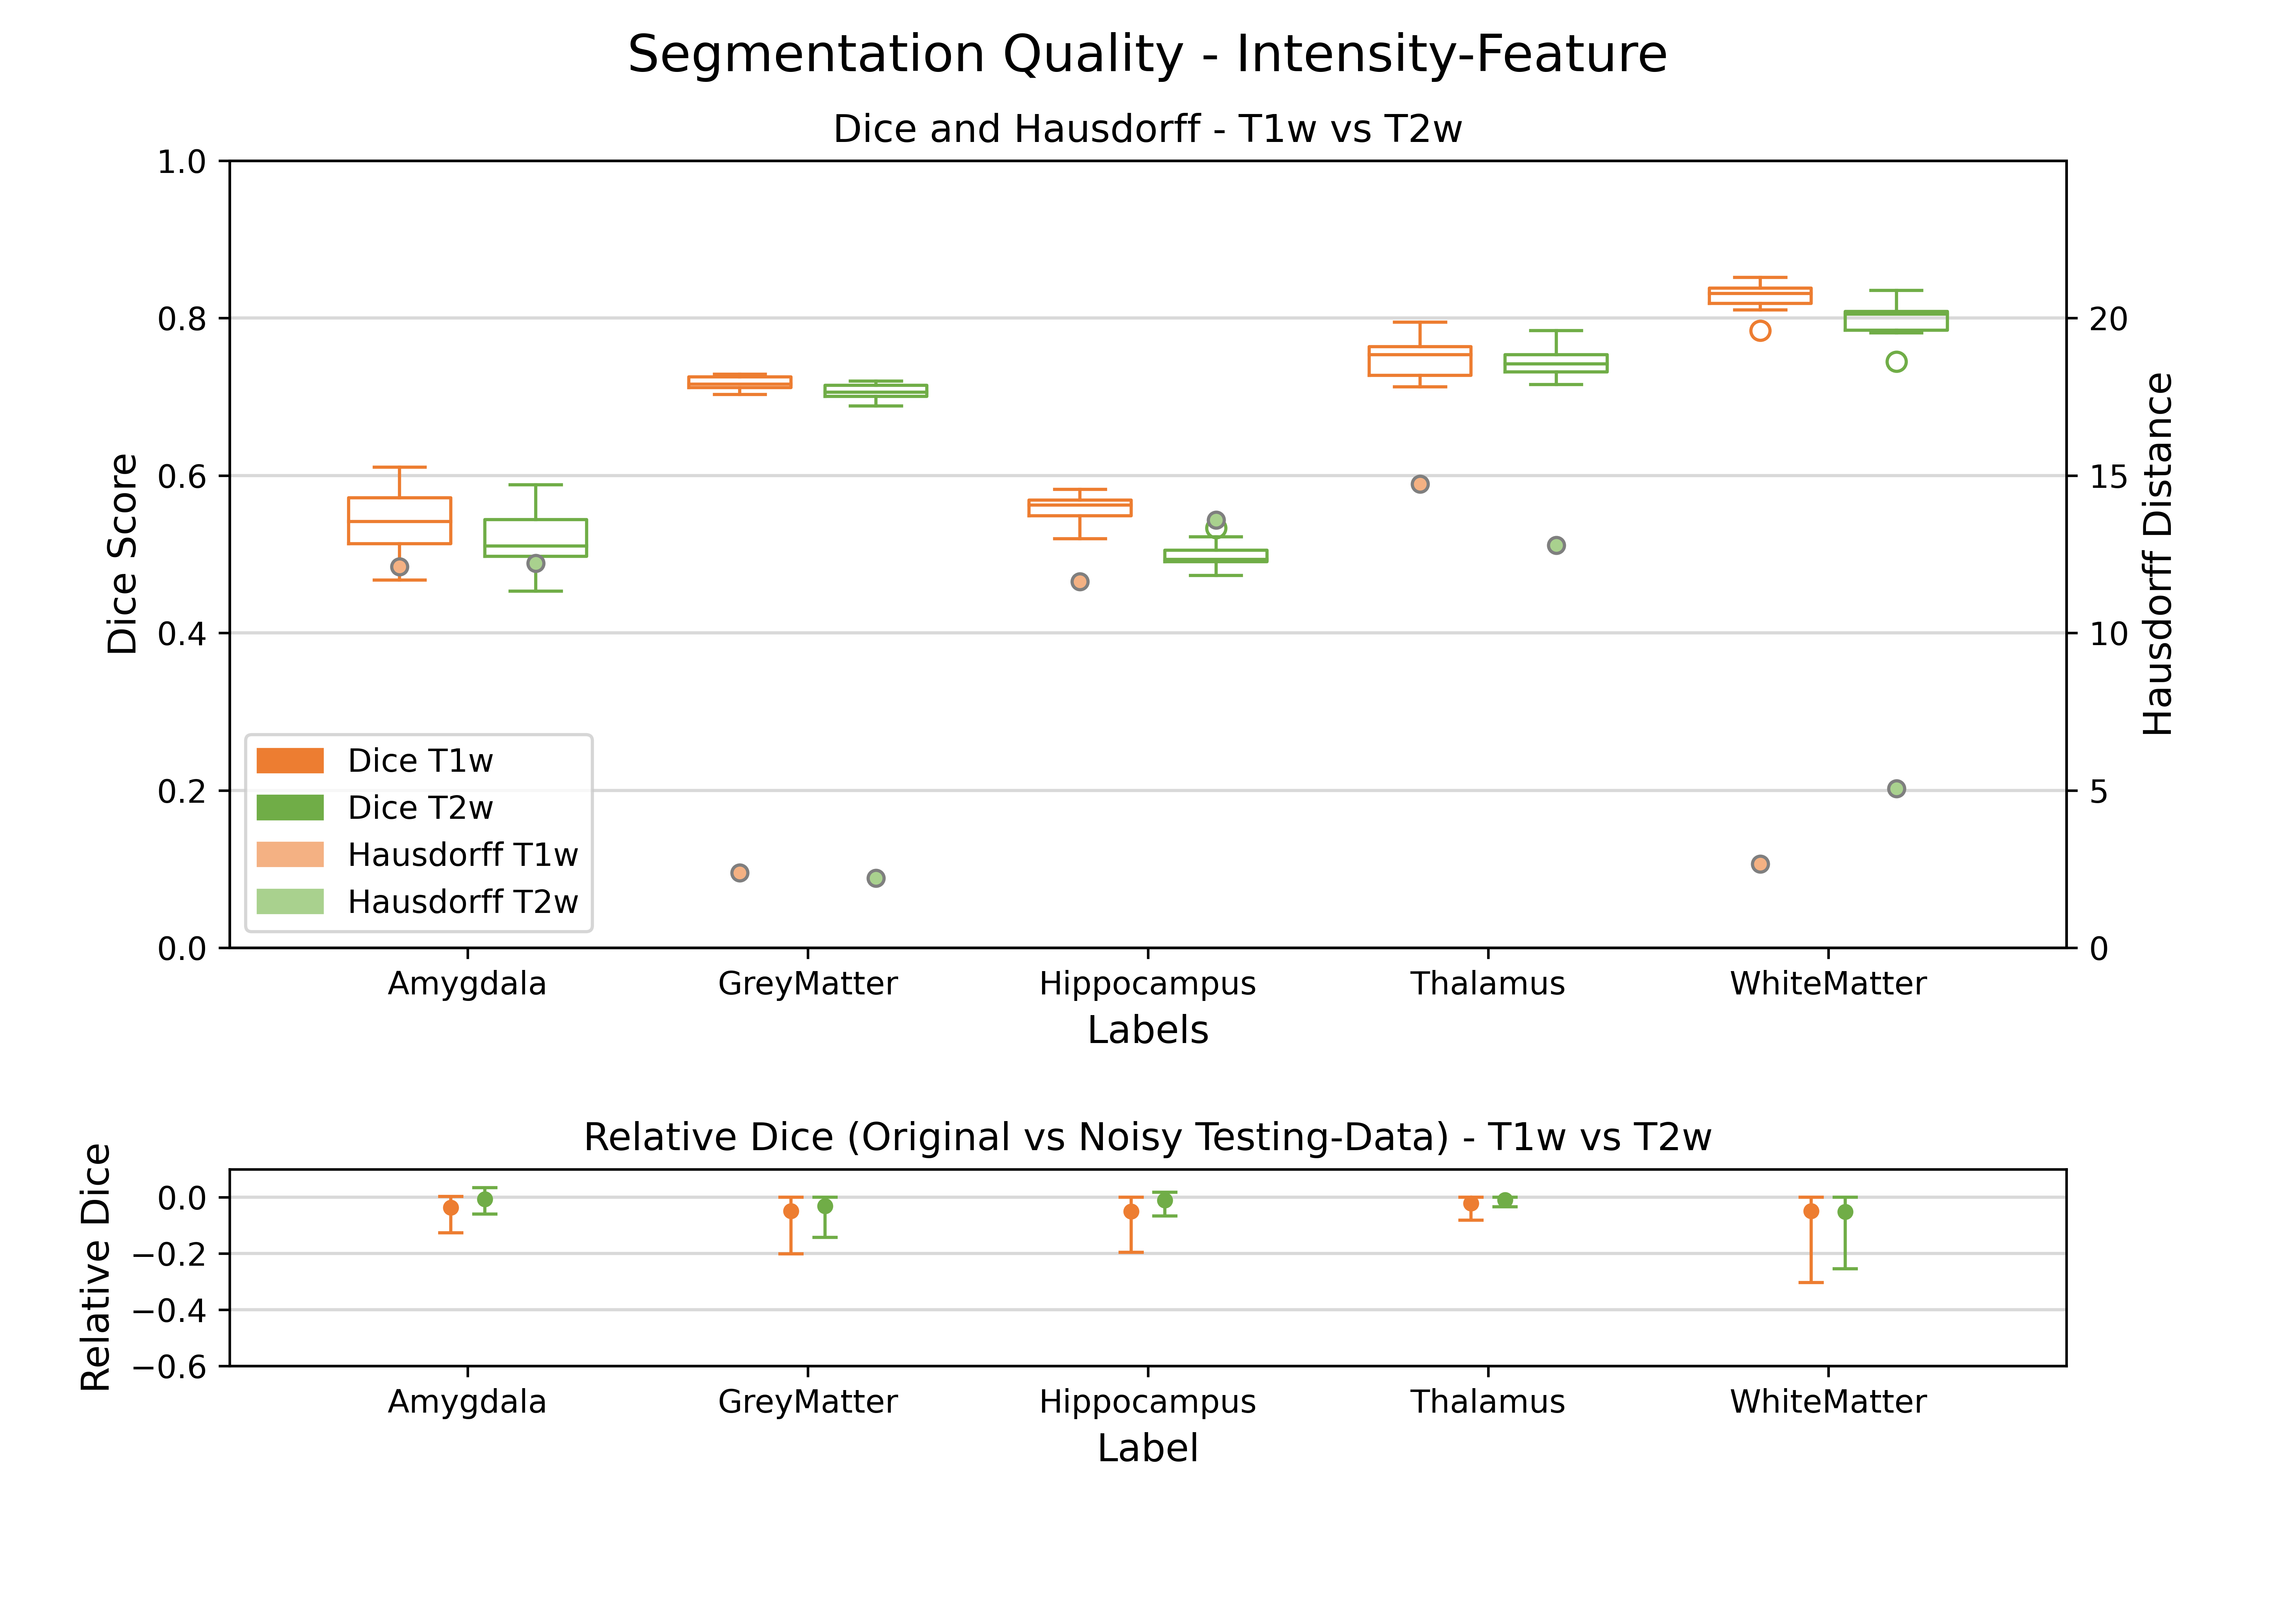
\includegraphics[width=0.9\textwidth, trim={0 15mm 0 10mm}, clip]{images/01_T1W_C_I_and_05_T2W_C_I.png}
      \caption{T1- and T2-weighted comparison with feature Intensity}
    \end{subfigure}
    \hspace{100mm}
    \begin{subfigure}
      \centering
      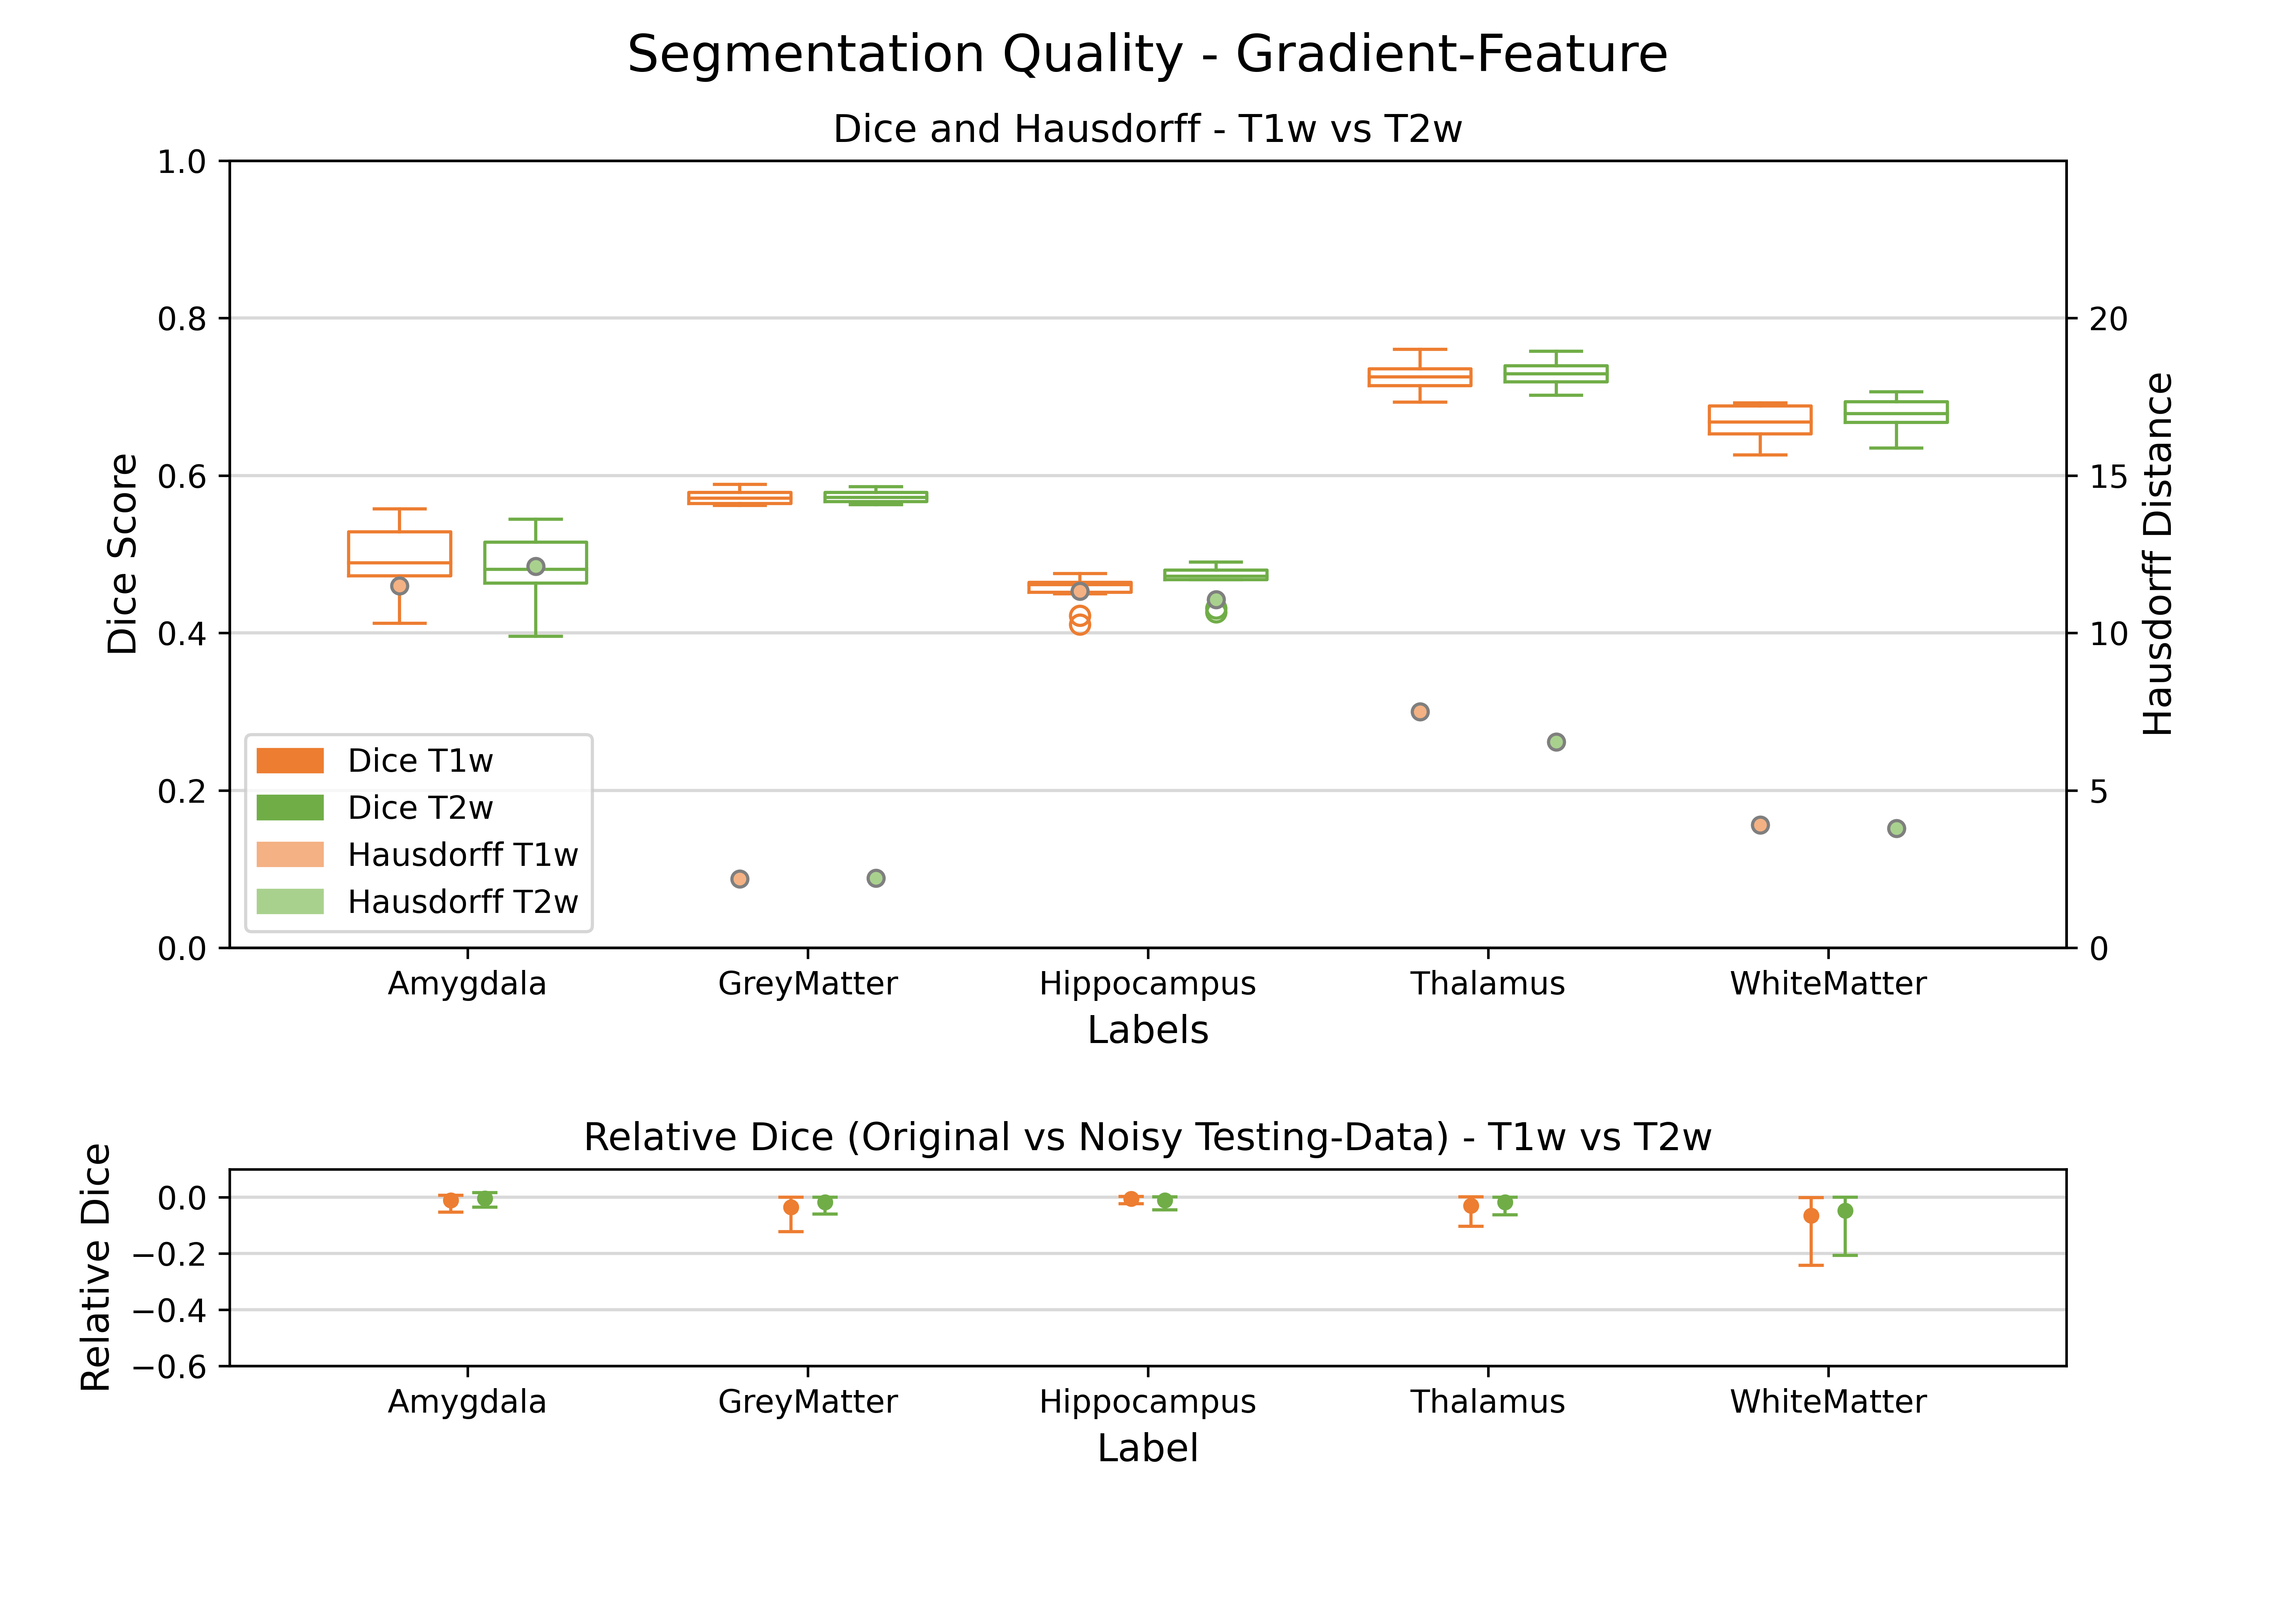
\includegraphics[width=0.9\textwidth, trim={0 15mm 0 10mm}, clip]{images/02_T1W_C_G_and_06_T2W_C_G.png}
      \caption{T1- and T2-weighted comparison with feature Gradient}
    \end{subfigure}
    %\caption{Three simple graphs}
    \label{fig:firstTwo}
\end{figure*}

\begin{figure*}
    \begin{subfigure}
      \centering
      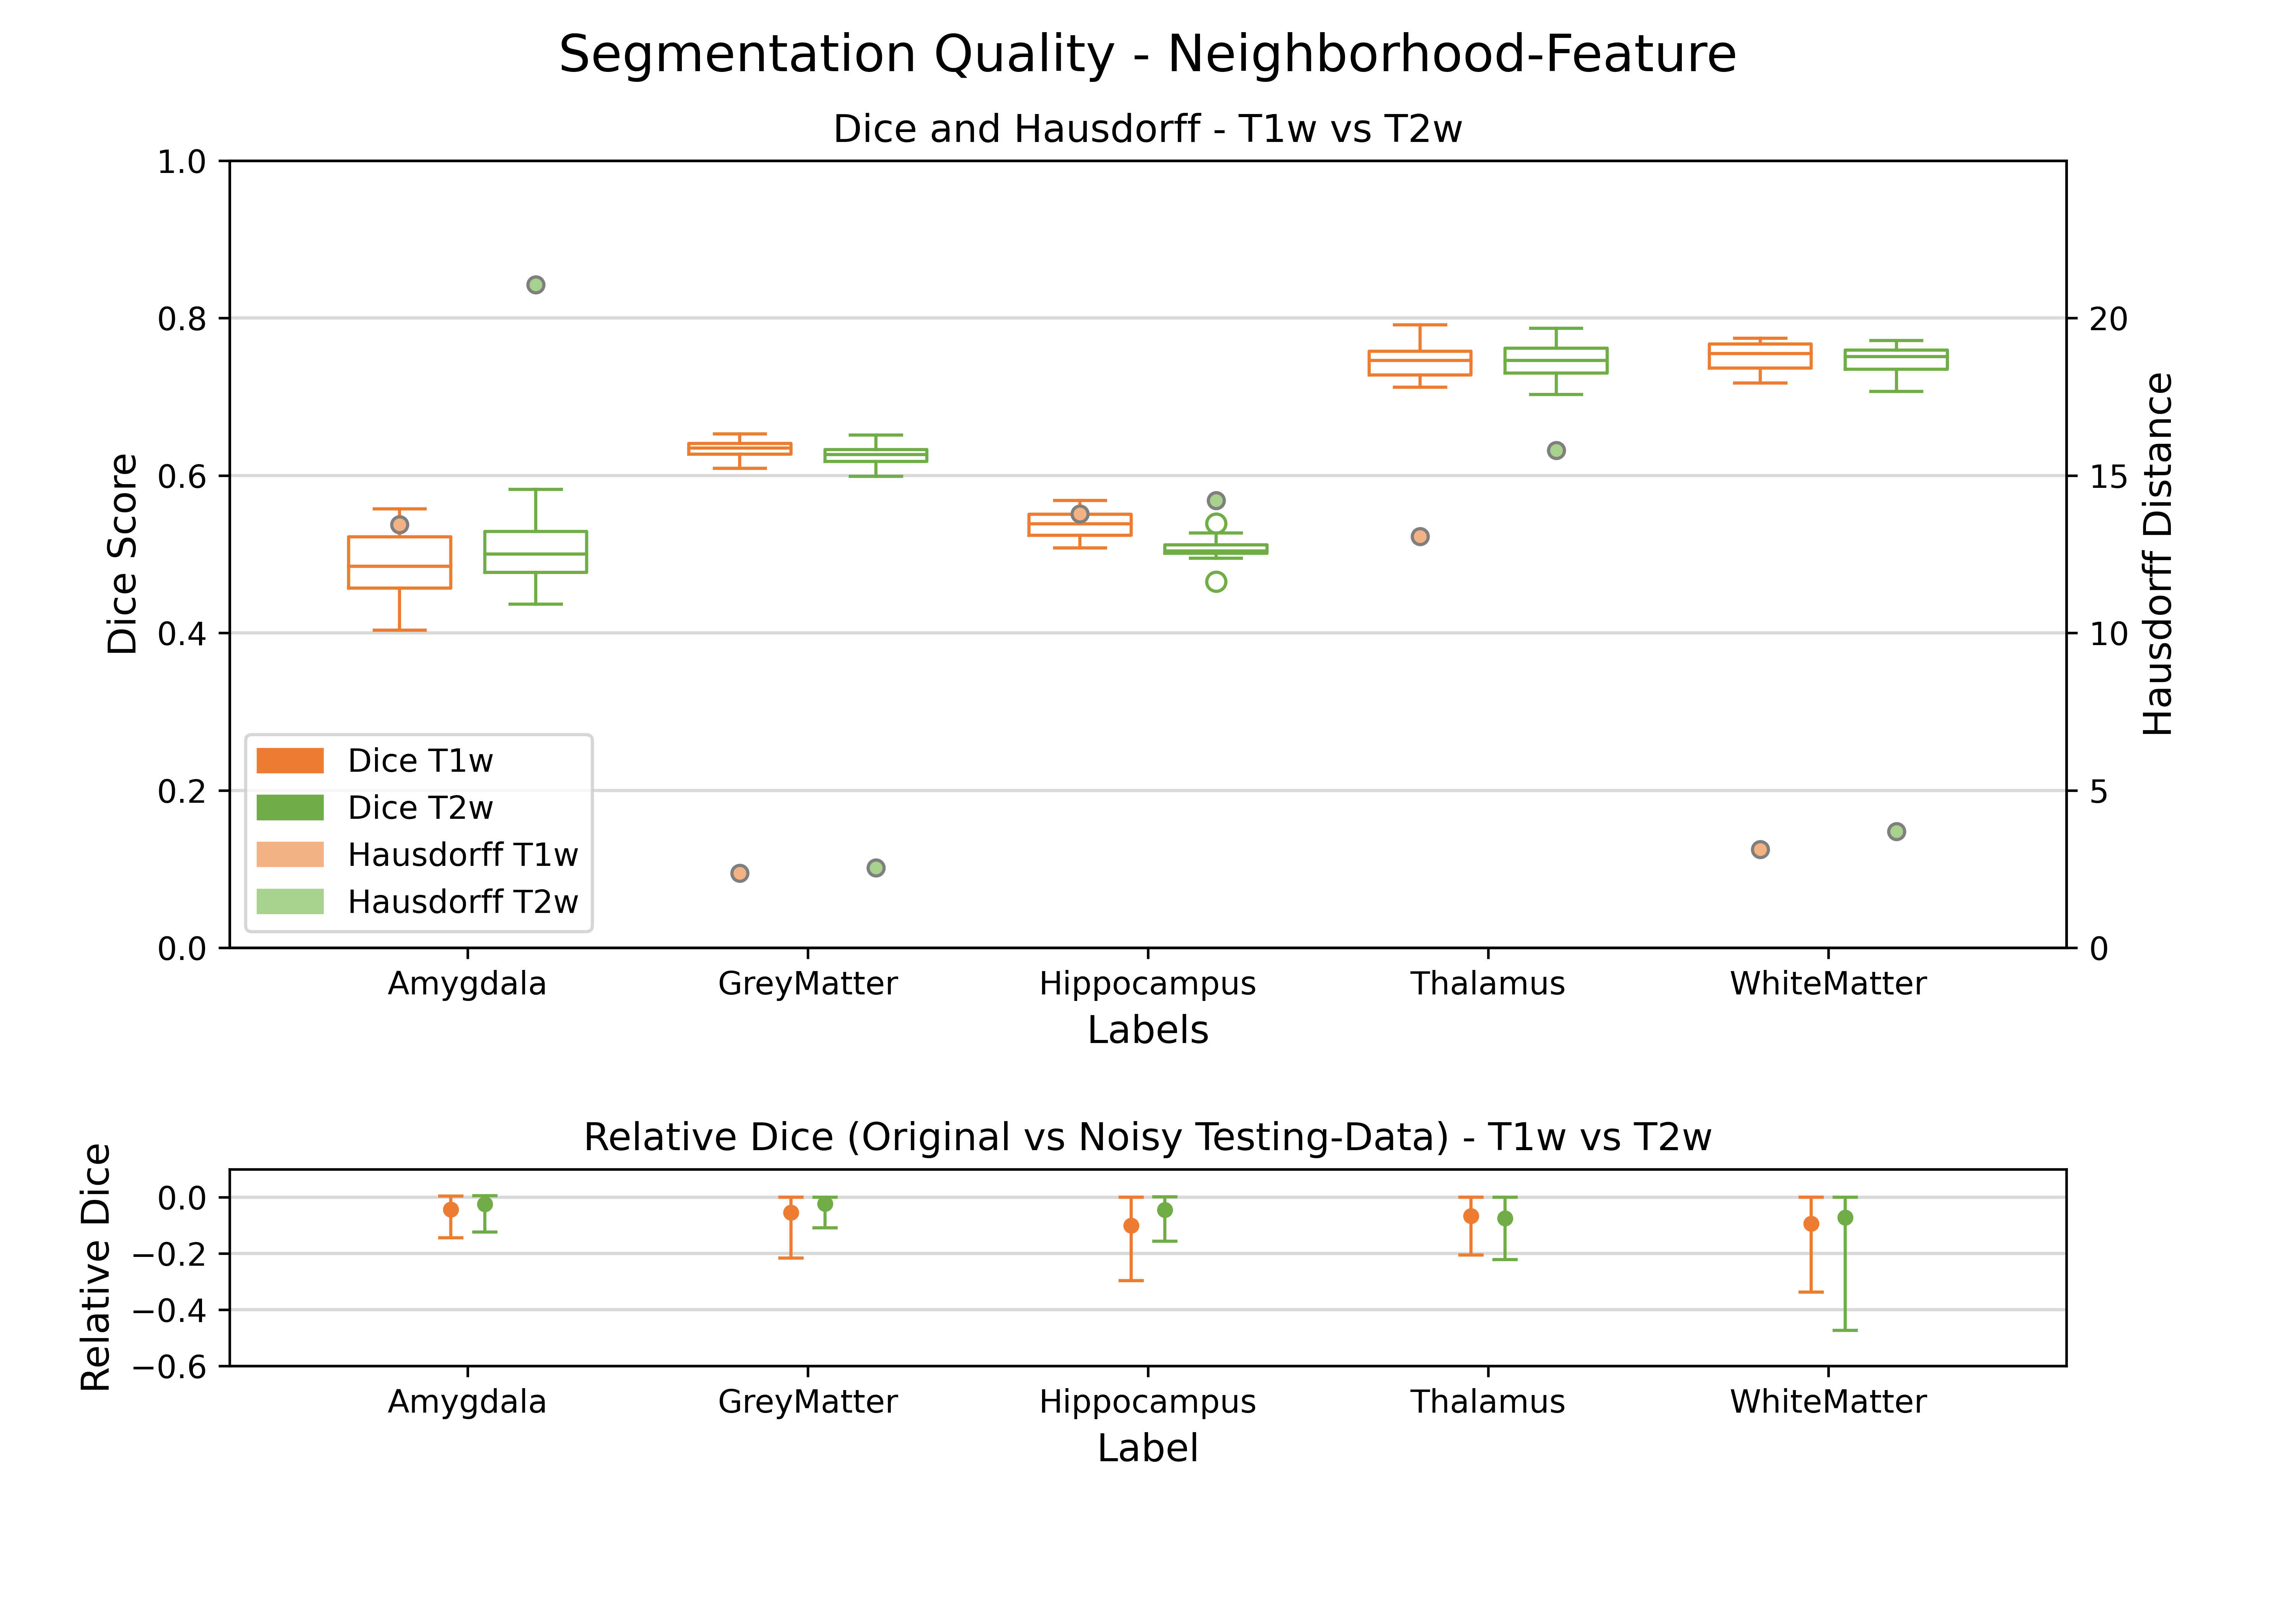
\includegraphics[width=0.9\textwidth, trim={0 15mm 0 10mm}, clip]{images/03_T1W_C_NH_and_07_T2W_C_NH.png}
      \caption{T1- and T2-weighted comparison with feature Neighbourhood}
    \end{subfigure}
    \hspace{100mm}
    \begin{subfigure}
      \centering
      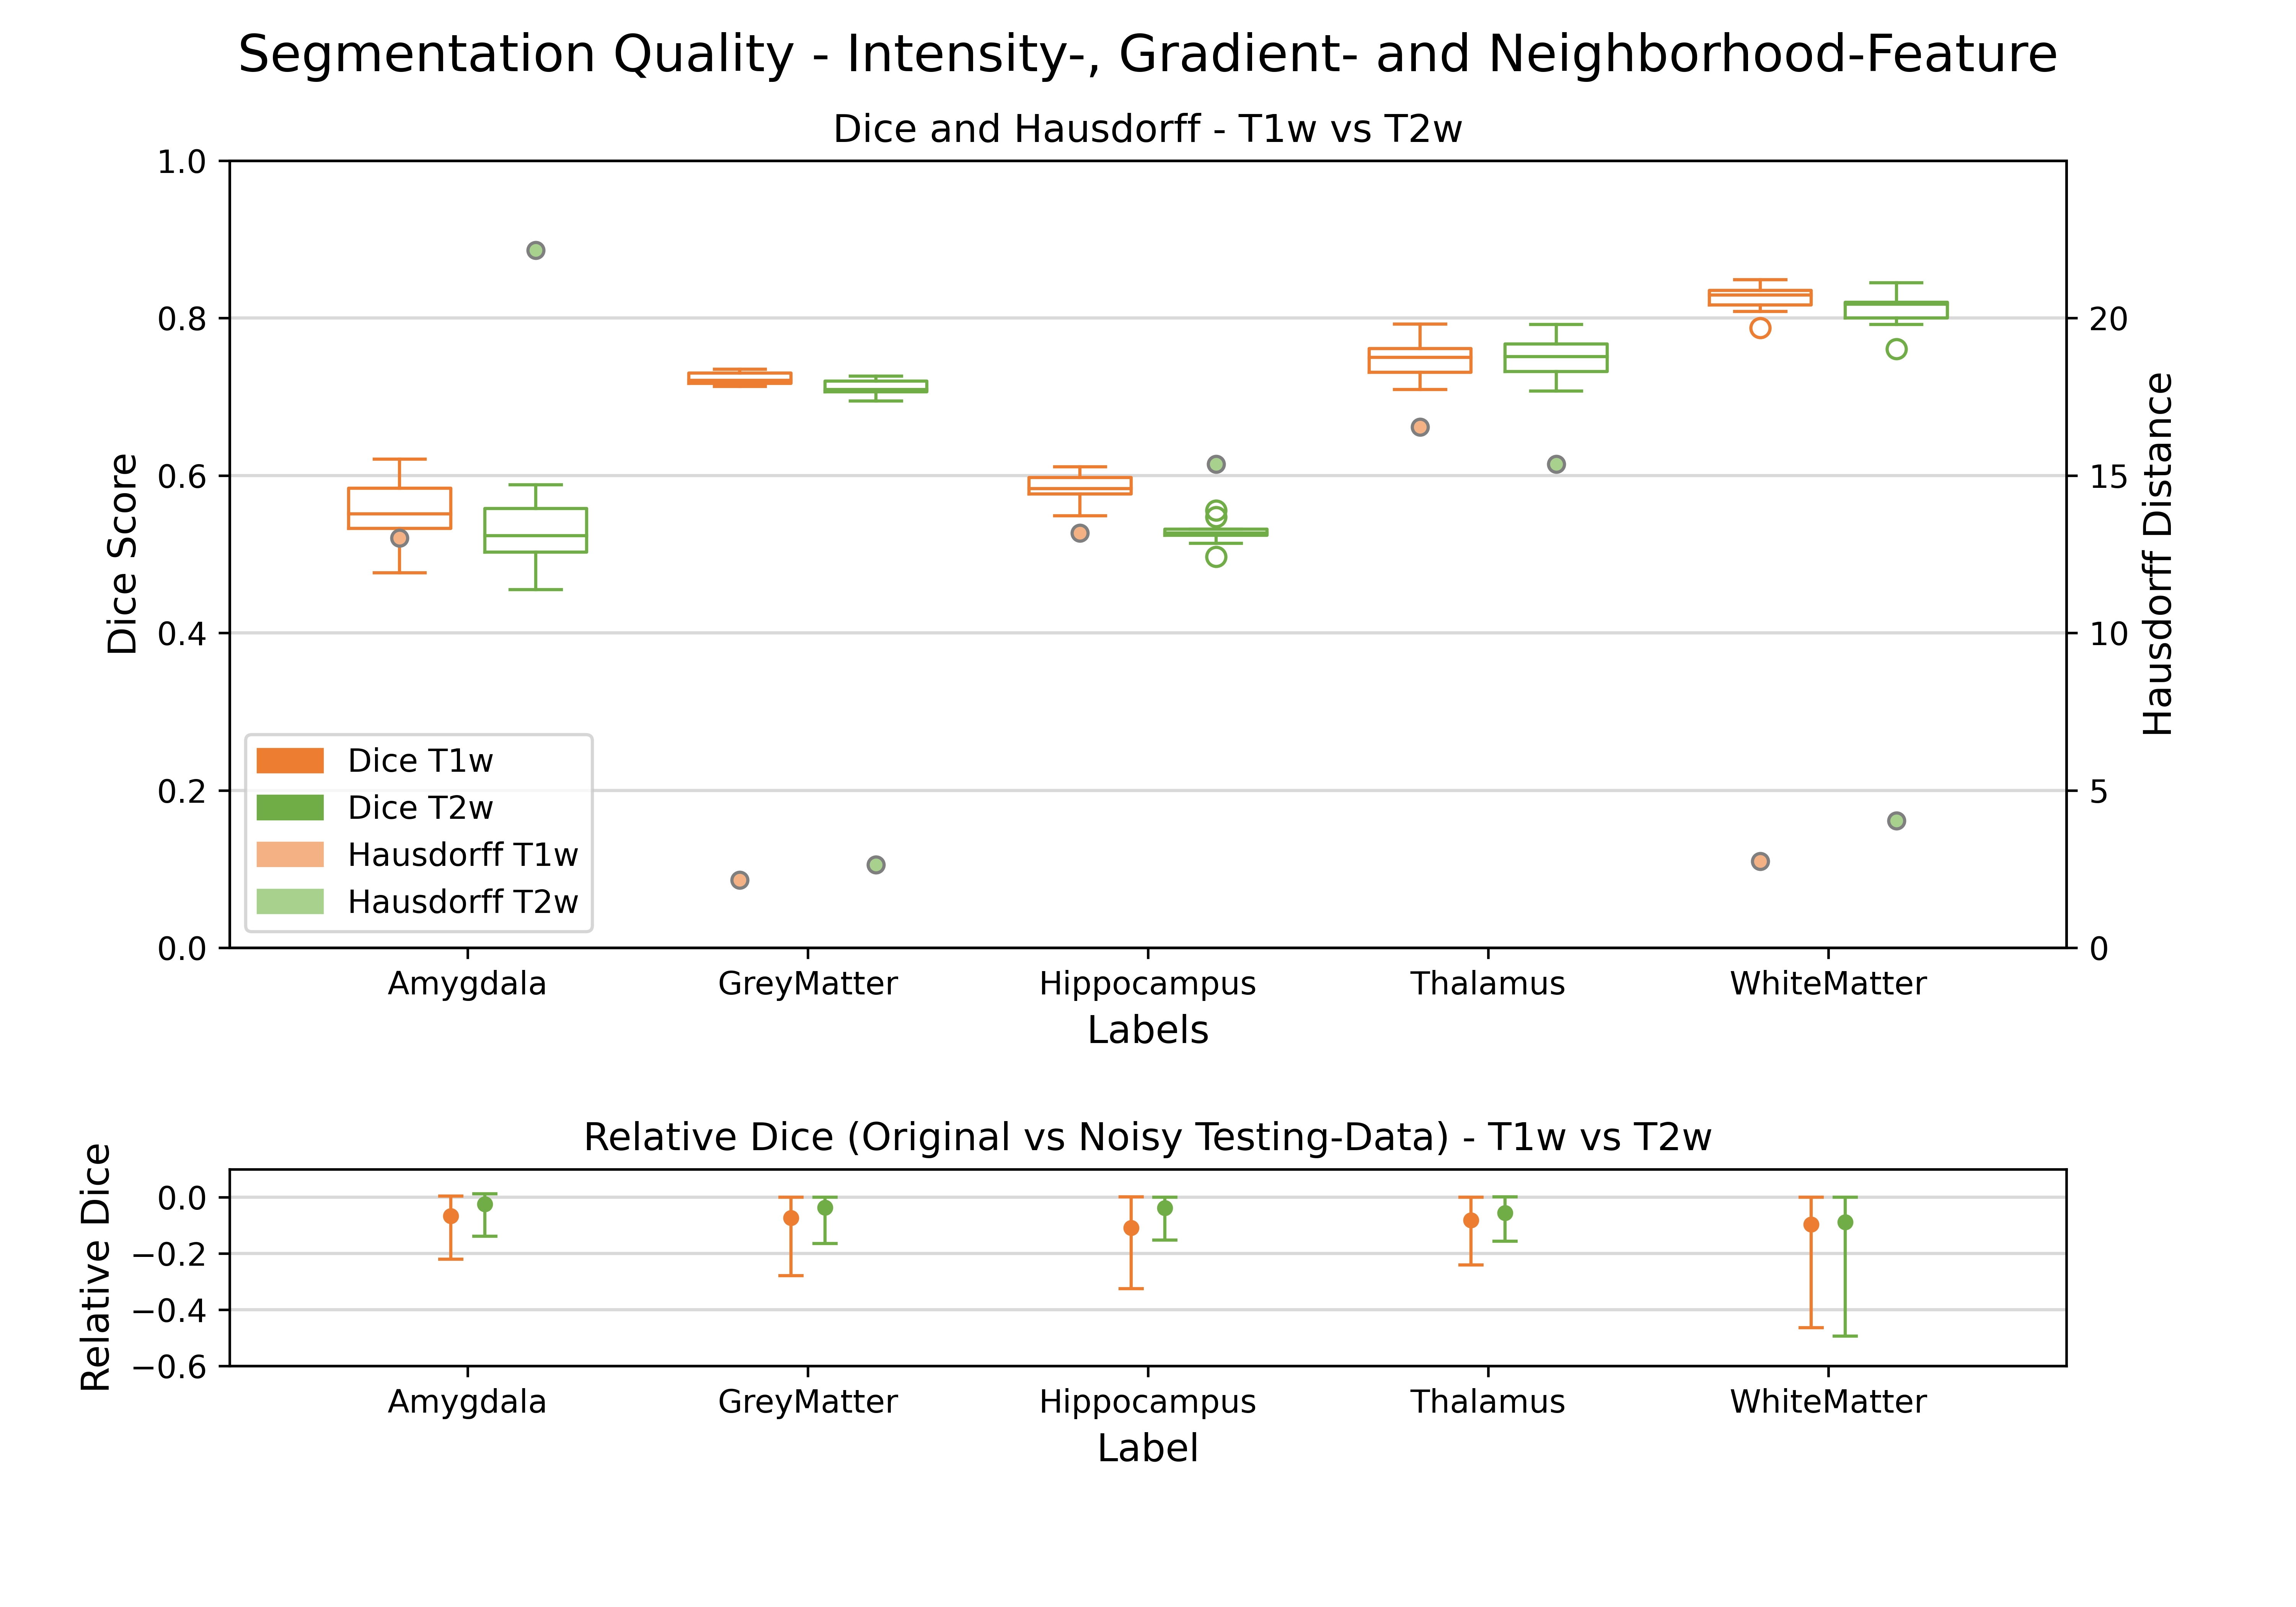
\includegraphics[width=0.9\textwidth, trim={0 15mm 0 10mm}, clip]{images/04_T1W_C_I_G_NH_and_08_T2W_C_I_G_NH.png}
      \caption{T1- and T2-weighted comparison with all three feature}
    \end{subfigure}
    %\caption{Three simple graphs}
    \label{fig:secondTwo}
\end{figure*}


\end{appendices}

\end{document}
